% Homework report template for courses lectured by Blaz Zupan.
% For more on LaTeX please consult its documentation pages, or
% read tutorials like http://tobi.oetiker.ch/lshort/lshort.pdf.
%
% Use pdflatex to produce a PDF of a report.

\documentclass[a4paper,11pt]{article}
\usepackage{a4wide}
\usepackage{fullpage}
\usepackage[toc,page]{appendix}
\usepackage[pdftex]{graphicx} % for figures
\usepackage{setspace}
\usepackage{color}
\definecolor{light-gray}{gray}{0.95}
\usepackage{listings} % for inclusion of Python code
\usepackage{hyperref}
\renewcommand{\baselinestretch}{1.2}

\lstset{ % style for Python code, improve if needed
language=Python,
basicstyle=\footnotesize,
basicstyle=\ttfamily\footnotesize\setstretch{1},
backgroundcolor=\color{light-gray},
}

\title{Homework Title}
\author{Student's Name (Student ID)}
\date{\today}

\begin{document}

\maketitle

\section{Introduction}

Report on the general goals of the homework or the assignment. Briefly state what was the problem that you were trying to solve. Use one paragraph of no more than 150 words. This part should alone describe the essence of the homework, allowing somebody not familiar with the homework assignment to understand what the homework was about.

\section{Data}

Most of the homeworks will rely on some data. Describe what data was used, where did it come from, and report on some basic statistics (e.g., the number and size of the sequences).

\section{Methods}

Report on the formal and computational methods that solve the problem from the homework. This can include the formal description of methods (equations),  outline of the algorithm or description of its  implementation in code. You can even include a short snippet that you find interesting and that is essential. If needed, you can illustrate your method in a figure or a diagram, like in Figure~\ref{fig-example}. Make sure you refer to all the figures and tables from the text in the report, as illustrated by an example in the previous sentence.

\begin{figure}[htbp]
\begin{center}
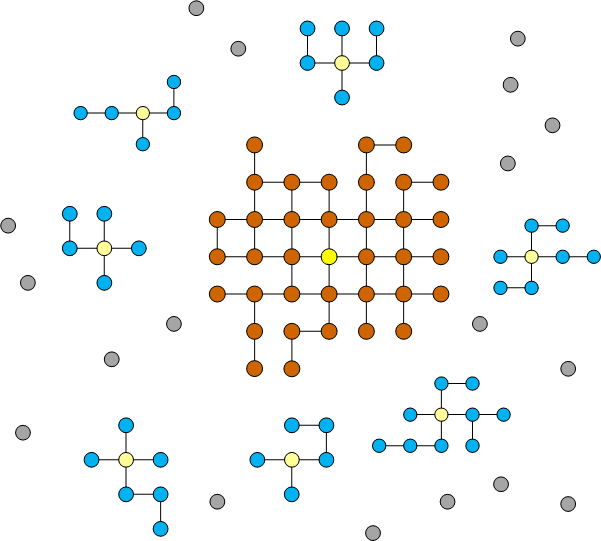
\includegraphics[scale=0.3]{figure-example.png}
\caption{Every figure should include a caption with a figure description.}
\label{fig-example}
\end{center}
\end{figure}

This part of the report can also include a short and illustrative code snippet. An example is provided below:

\begin{lstlisting}
def fib(n):
    if n == 0:
        return 0
    elif n == 1:
        return 1
    else:
        return fib(n-1) + fib(n-2)
\end{lstlisting}

\section{Results}

Report on results and provide short, preferably one-paragraph long discussion. Depending on a homework, you can present quantitative results of your experiments in the table (see Table~\ref{tab1}). Provide reference to every table from main text, just like we did in the previous sentence. Notice that Tables should not include vertical lines, and should include horizontal lines only to separate the header from the content and to indicate the end of the table.

\begin{table}[htbp]
\caption{Data attributes and their values.}
\label{tab1}
\begin{center}
\begin{tabular}{llp{4cm}}
\hline
name & domain  & description \\
\hline
price & [0, 500] & item price in EUR\\
weight & [1, 1000] & item weight in dag \\
quality & [poor|acceptable|good] & quality of an item \\
\hline
\end{tabular}
\end{center}
\end{table}

\subsection{Structure of the Report}

If needed, this section could be structured. If the homework is composed of several tasks (or questions), the report on each of them could be presented in a separate section (use \LaTeX's {\tt \\subsection} command). The report of the results should be brief. If really needed, any  more extensive results of your homework should be reported in the Appendix (see Appendix~\ref{app-res} and~\ref{app-code}).

\subsection{Paragraphs}

A short note on the paragraphs: these are introduced in \LaTeX\ by an empty line before the paragraph.

\subsection*{Honor Code}

% The following paragraph of your report should be included as is - do % not change it.

My answers to homework are my own work. I did not make solutions or code available to anyone else. I did not engage in any other activities that will dishonestly improve my results or dishonestly improve/hurt the results of others.

\appendix
\appendixpage
\section{\label{app-res}Detailed Results of Experiments}

If you consider that report should include detailed results in the form of tables and figures, include them here. Essential results should be included in the main part of the report (section on results).

\section{\label{app-code}Program Code}

Each homework will require a development of specific implementation in Python. Most of the homeworks will request that this code is submitted as a separate document. Only if this is not the case, that is, the homework requests that you provide the entire code in the report, do so in this appendix. Following is an example, and includes a part of code from Orange (\url{http://www.biolab.si/orange}) that implements 
clustering.

\begin{lstlisting}
import random
import Orange

data_names = ["iris", "housing", "vehicle"]
data_sets = [Orange.data.Table(name) for name in data_names]

print "%10s %3s %3s %3s" % ("", "Rnd", "Div", "HC")
for data, name in zip(data_sets, data_names):
    random.seed(42)
    km_random = Orange.clustering.kmeans.Clustering(data, centroids = 3)
    km_diversity = Orange.clustering.kmeans.Clustering(data, centroids = 3,
        initialization=Orange.clustering.kmeans.init_diversity)
    km_hc = Orange.clustering.kmeans.Clustering(data, centroids = 3,
        initialization=Orange.clustering.kmeans.init_hclustering(n=100))
    print "%10s %3d %3d %3d" % (name, km_random.iteration, \
    km_diversity.iteration, km_hc.iteration)
\end{lstlisting}

\end{document}

